\documentclass[aspectratio=169]{beamer}
\usetheme{Copenhagen}
%% Remove draft for real article, put twocolumn for two columns
\usepackage[utf8]{inputenc}

\newcommand{\vectorproj}[2][]{\mathrm{proj}_{\vect{#1}}\vect{#2}}
\newcommand{\vectorcomp}[2][]{\mathrm{comp}_{\vect{#1}}\vect{#2}}
\newcommand{\vect}{\mathbf}
%% commentary bubble
\newcommand{\SV}[2][]{\sidenote[colback=green!10]{\textbf{SV\xspace #1:} #2}}

%% Title 
\title{ Multivariable Calculus \\ Day 1}
\institute{Fulbright University Vietnam}
%\author[1]{Co-author}
\author{Truong-Son Van}
\date{Spring 2024}

\begin{document}

\maketitle


\begin{frame}
    \frametitle{Introduction}
    \begin{itemize}
        \item Instructor: Truong-Son Van
        \item Time: M \& W, 9:45a-11:15a
        \item Office hours: TBD 
        \item TA:  TBD
    \end{itemize}
\end{frame}

\begin{frame}
    \frametitle{Overview}
    \begin{itemize}
        \item Logistics
        \item Getting started 
    \end{itemize}
\end{frame}

\begin{frame}
    \frametitle{Single variable vs. Multivariable}

\end{frame}

\begin{frame}
    \frametitle{What's the point?}
    What do you think is the function that create this graph?
    \centering
    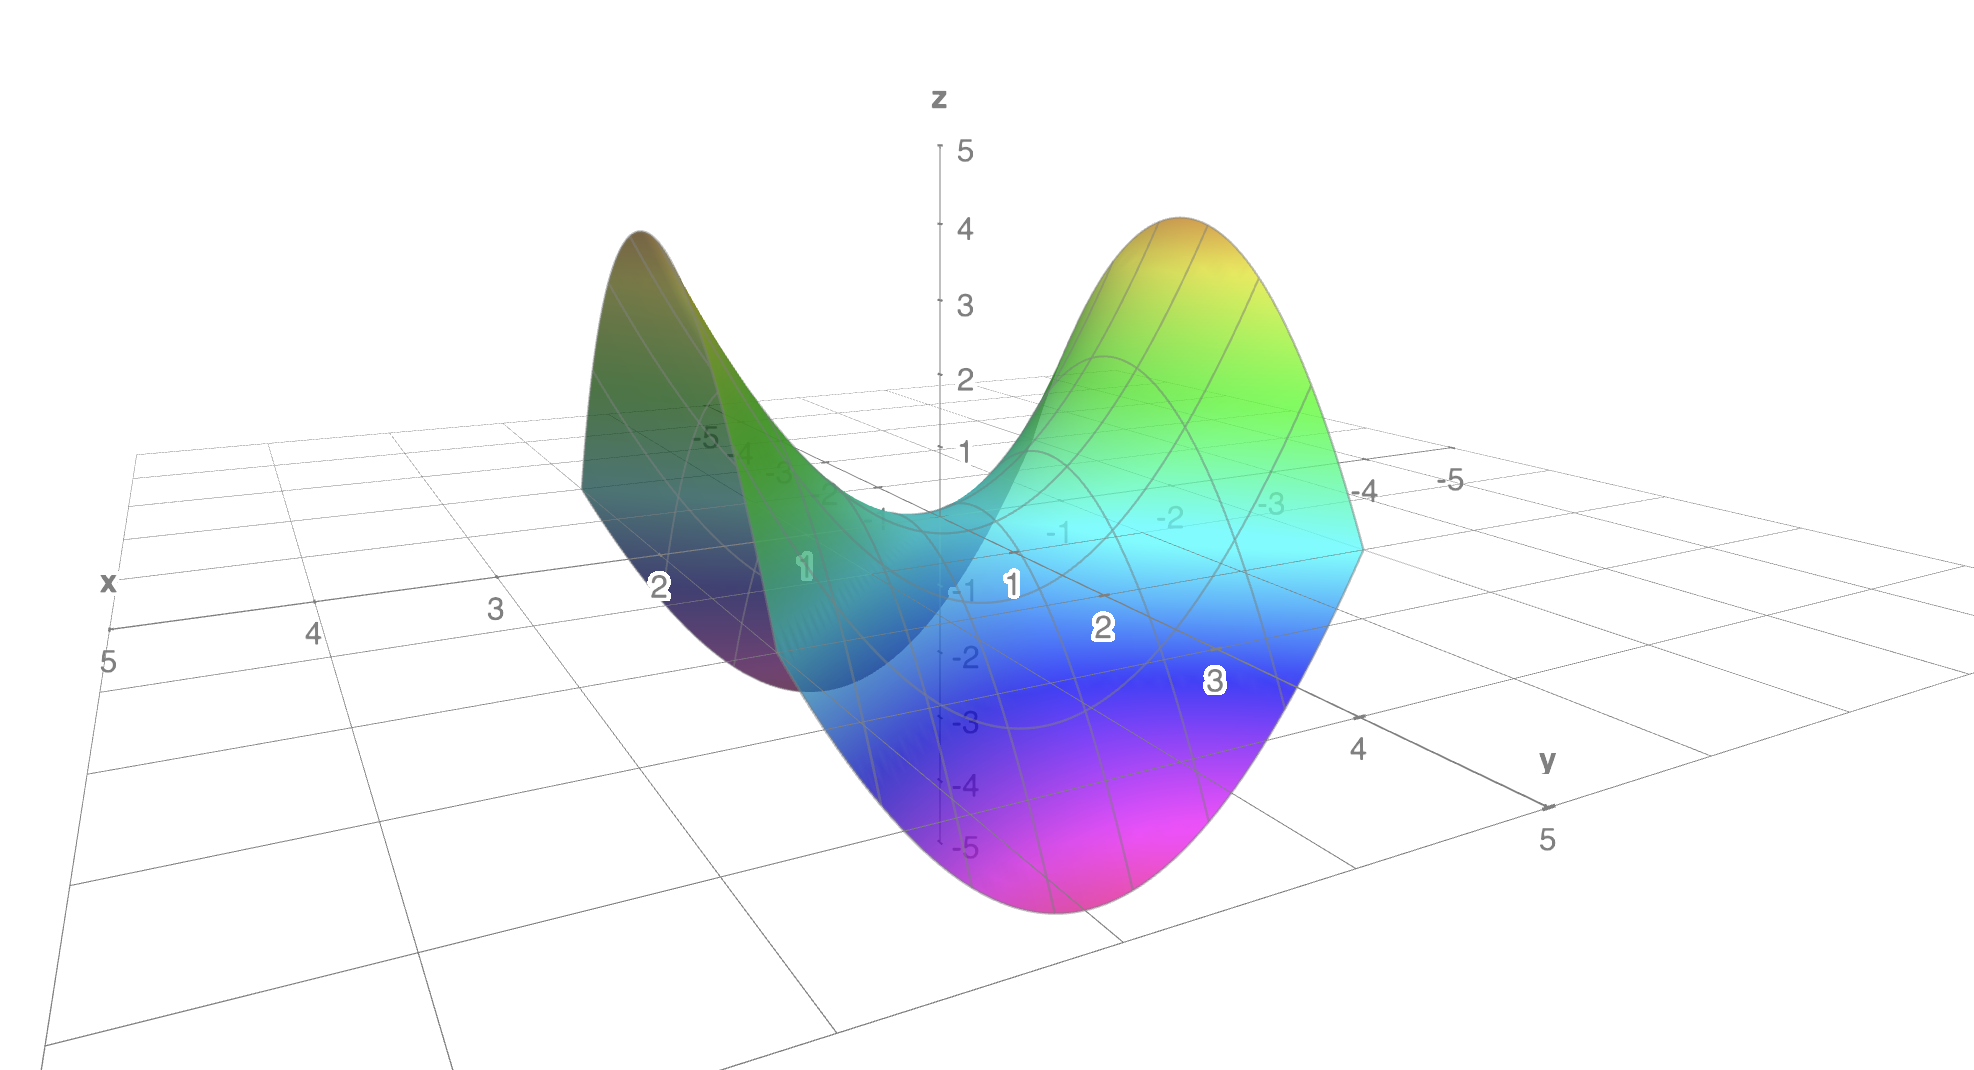
\includegraphics[width=0.7\textwidth]{saddle}
\end{frame}

\begin{frame}
    \frametitle{What's the point?}
    Life is a function with many variables \pause

    \centering
    
\includegraphics[height=0.5\textheight]{sad}
\end{frame}

\begin{frame}
    \frametitle{What will you learn?}
    \url{https://www.tsvan.xyz/MultiCalc}
\end{frame}

\begin{frame}
    \frametitle{Final word on style}
    \begin{itemize}
        \item Certain things in math have to be delivered while writing.
        \item So, I'll deliver my lectures by writing on the iPad / whiteboard.
        \item Slides/brief notes just contain key points.
        \item It is your responsibility to update your notes to include the details I speak in class.
    \end{itemize}

\end{frame}



\end{document}
